%\documentclass[a4paper]{article}
%\usepackage{graphicx}
%\usepackage{caption}
%\usepackage{subcaption}
%\begin{document}


\section{Results}
	This section will present the results of applying homomorphic filtering
	on an image. Also provided is some experiments with different images
	and filters not used in the book, as to test if this method could yield
	better or worse results in different types of information depicted.
	\subsection{Results on the image provided with the project}
		The image provided with the project depicts a forest scenery. %include picture
		As seen in figure [INSERT IMAGE HERE] it contains a mix of both low 
		and high frequencies. In figure [INSERT IMAGE HERE] the major areas of 
		the different frequencies can be seen. The filter used in this project was
		the gaussian high-pass filter detailed in the course book on pp. 314; 
		%
		\begin{equation}
		\label{eqn:gaussian_filter}
			H(u,v) = \left( \gamma_H - \gamma_L \right) \left[ 1 - e^{c \left[D^2(u,v)/D_0^2\right]}\right] + \gamma_L 
		\end{equation}
		 %
		This filter has additional $\gamma$-parameters added in order to tweak
		the filter in regard to illumination and reflection. The $\gamma_L$ parameter
		will define the amount of suppression of the low frequencies; a lower $\gamma_L$
		will keep more low frequencies. Likewise a large value of the $\gamma_H$ parameter 
		will emphasize the high frequencies. As an example, examine figure~\ref{fig:gamma_diff}.
		\begin{figure}[h!]
        \centering
        \begin{subfigure}[b]{0.6\textwidth}
                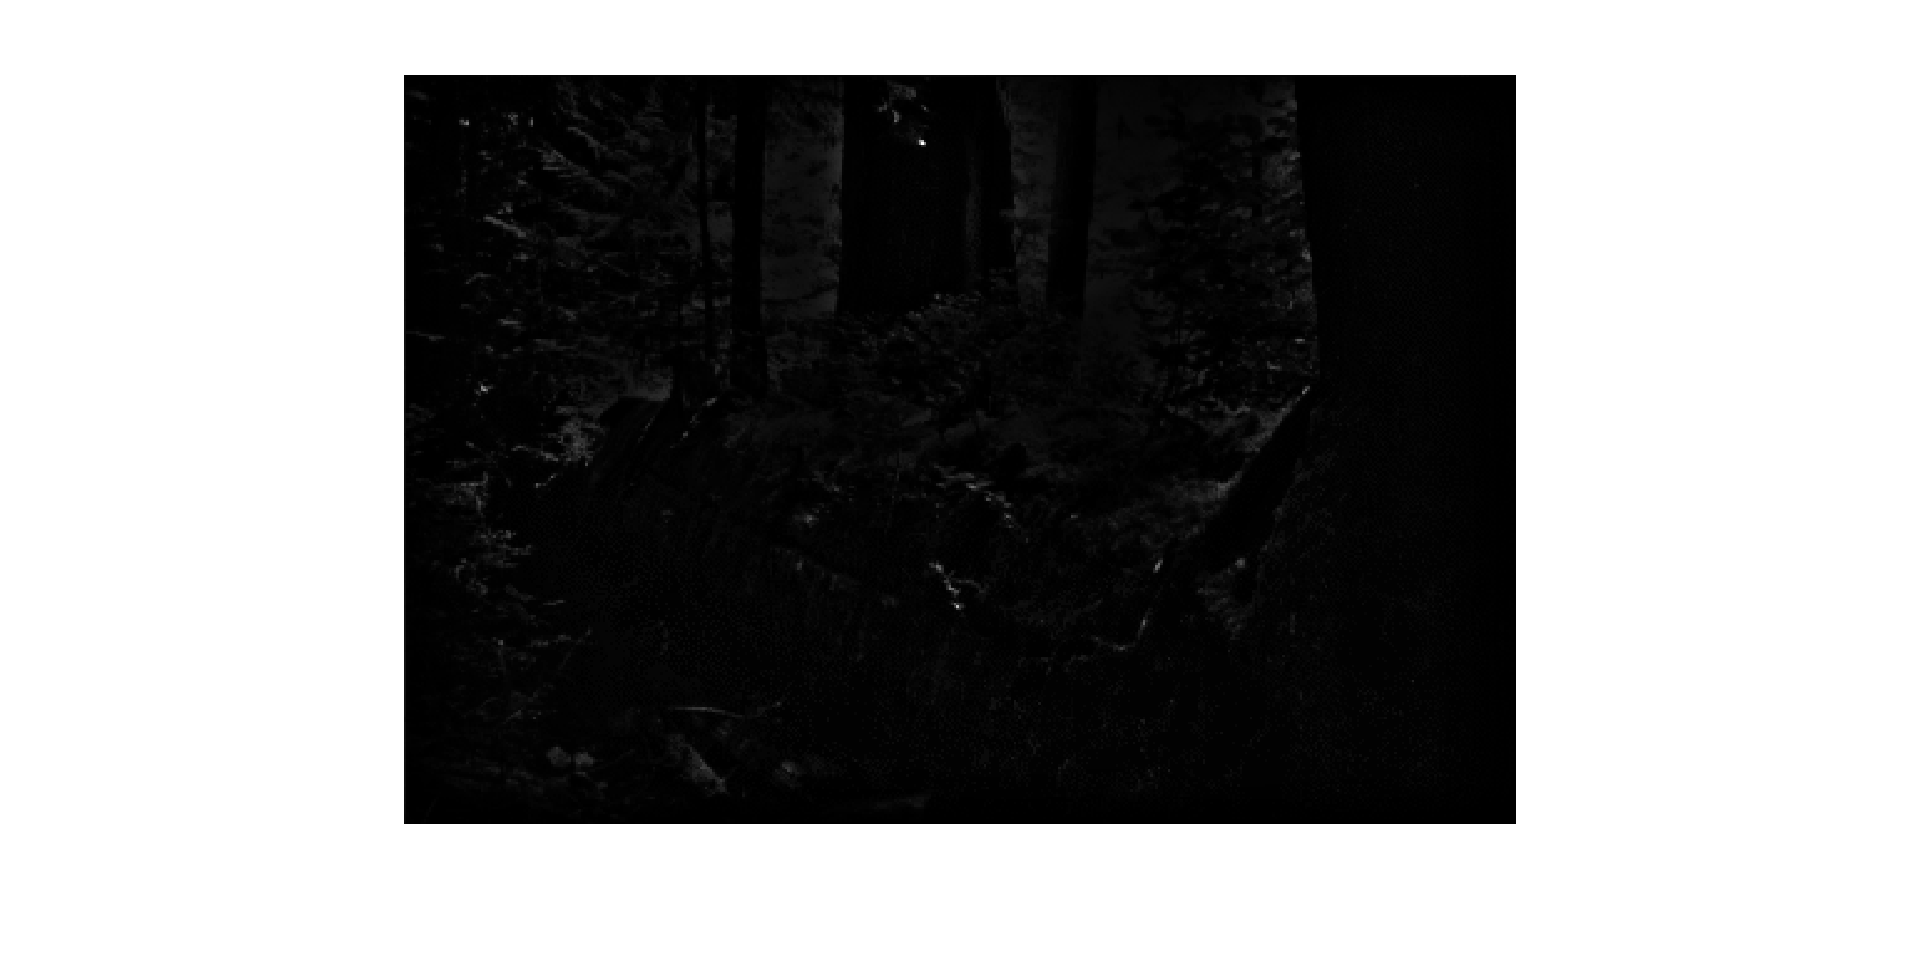
\includegraphics[width=\textwidth]{pics/gamma_difference_emph_lowfreq.png}
                \caption{$\gamma_L = 0.1,~\gamma_H = 2$}
                \label{fig:gamma_l_emph}
        \end{subfigure}%
        \begin{subfigure}[b]{0.6\textwidth}
                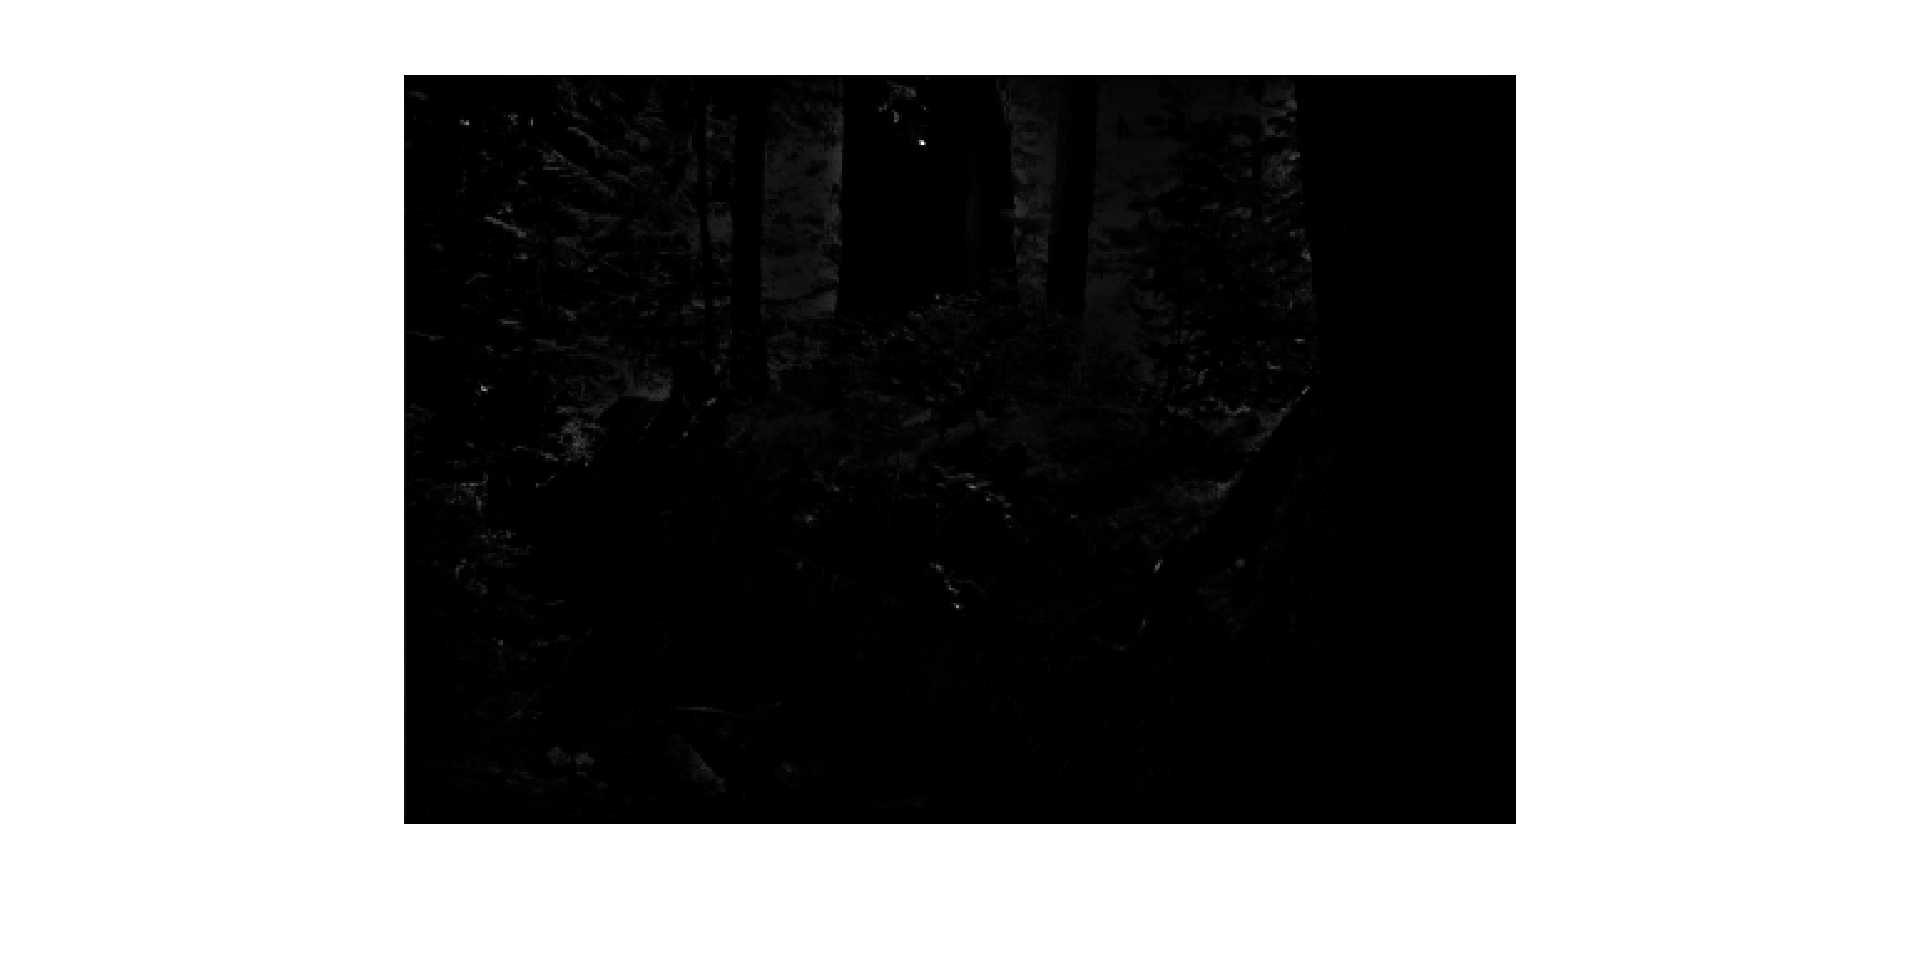
\includegraphics[width=\textwidth]{pics/gamma_difference_no_emph_lowfreq.png}
                \caption{$\gamma_L = 0.9,~\gamma_H = 2.8$}
                \label{fig:gamma_l}
        \end{subfigure}
        \caption{The difference between $\gamma_L$ and $\gamma_H$ is kept intact}\label{fig:gamma_diff}
		\end{figure}
		In figure~\ref{fig:gamma_l_emph} it can be seen that the lower set~$\gamma_L$ will preserve
		more of the low frequencies (illumination), such as the details on the stems of the trees
		and some of the foliage. The difference between the $\gamma$-parameters were fixed in
		this test for consistency, but the $\gamma_L$ parameter will still change the image
		as it is added to the filter. % Märklig formulering
		\\
		\\
		Various $\gamma_l$ and $\gamma_h$ paramaters has been tried out with various results.
		
	
	\subsection{Experiments with different images}

%\end{document} 